\documentclass[11pt,a4paper]{article}

\usepackage[margin=2.2cm]{geometry}
\usepackage[T1]{fontenc}
\usepackage{lmodern}
\usepackage{microtype}
\usepackage{xcolor}
\usepackage{booktabs}
\usepackage{tabularx}
\usepackage{ltablex}
\keepXColumns
\usepackage{enumitem}
\usepackage{listings}
\usepackage{tikz}
\usetikzlibrary{arrows.meta,positioning,shapes.geometric}
\usepackage[most]{tcolorbox}
\usepackage{titlesec}
\usepackage{needspace}
\usepackage{fancyhdr}
\usepackage[colorlinks=true,linkcolor=accent,urlcolor=accent]{hyperref}

\definecolor{accent}{HTML}{1F5FAD}
\definecolor{soft}{HTML}{EEF3FA}
\definecolor{codebg}{HTML}{F6F8FA}
\definecolor{codekw}{HTML}{8A2BE2}
\definecolor{codestr}{HTML}{0A7D32}
\definecolor{codecom}{HTML}{6A737D}
\definecolor{metrored}{HTML}{D32F2F}
\definecolor{metroblue}{HTML}{1565C0}
\definecolor{metrogreen}{HTML}{2E7D32}

\titleformat{\section}{\Large\bfseries\color{accent}}{\thesection}{0.6em}{}
\titleformat{\subsection}{\large\bfseries}{\thesubsection}{0.6em}{}
\setlength{\parskip}{0.5em}
\setlength{\parindent}{0pt}
\setlist{itemsep=0.2em,topsep=0.3em}

\pagestyle{fancy}
\fancyhf{}
\fancyhead[L]{\small\color{codecom}RouteMate AI --- Beginner's Guide}
\fancyhead[R]{\small\color{codecom}\thepage}
\renewcommand{\headrulewidth}{0.3pt}

\lstset{
  basicstyle=\ttfamily\small,
  backgroundcolor=\color{codebg},
  frame=single, rulecolor=\color{codebg},
  keywordstyle=\color{codekw}\bfseries,
  stringstyle=\color{codestr},
  commentstyle=\color{codecom}\itshape,
  showstringspaces=false,
  breaklines=true,
  columns=fullflexible,
  keepspaces=true,
  upquote=true,
  xleftmargin=0.4em, xrightmargin=0.4em,
  aboveskip=0.6em, belowskip=0.6em
}
\lstdefinestyle{shell}{language=bash,keywordstyle=\color{black}}

\newtcolorbox{tip}[1][Tip]{colback=soft,colframe=accent,boxrule=0.6pt,arc=2pt,
  left=6pt,right=6pt,top=4pt,bottom=4pt,fonttitle=\bfseries\small,title=#1}

\newcommand{\file}[1]{\texttt{\color{accent}#1}}

\begin{document}

\begin{center}
  {\Huge\bfseries RouteMate \textcolor{accent}{AI}}\\[0.4em]
  {\Large A beginner's guide to what we built, how, and how to run it}\\[0.6em]
  {\small Codegnan Python Group Project \quad$\cdot$\quad Batch PFS-66}
\end{center}

\vspace{0.4em}

\begin{tip}[Who this guide is for]
You know basic Python (variables, lists, dictionaries, functions, loops) and want to
understand our project well enough to run it, explain it in the viva, and change it.
You do \emph{not} need to know graph theory, Flask or AI beforehand; every idea is
introduced from scratch.
\end{tip}

\tableofcontents

\section{What is RouteMate AI?}

RouteMate AI is a website that plans trips on the \textbf{Hyderabad Metro}.
You type a question in normal English (or Telugu or Hindi), for example:

\begin{center}
\itshape ``I'm at Ameerpet, need to reach Hitech City before 10, don't want to change trains much''
\end{center}

and the app answers with:
\begin{itemize}
  \item which trains to take, where to change, and at what time to leave;
  \item how long the trip takes, how many stops, and the fare in rupees;
  \item the route drawn on a map, plus a short friendly explanation.
\end{itemize}

The network in the app is real: \textbf{3 lines} (Red, Blue, Green) and \textbf{57 stations},
with the official fare chart (Rs.\ 11 to Rs.\ 69).

\subsection*{The one idea to remember}

\begin{tip}[The AI never picks the route]
The AI (Google Gemini) does only two jobs: it \textbf{reads} your question and it
\textbf{explains} the answer. The route itself is always computed by \emph{our own Python
code} using classic algorithms. So the answer is always a real, correct route, never a guess.
\end{tip}

\begin{center}
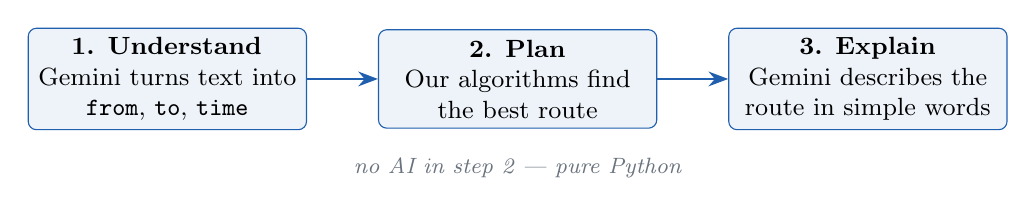
\begin{tikzpicture}[
  box/.style={draw=accent,fill=soft,rounded corners=3pt,align=center,minimum height=1.25cm,text width=3.3cm,font=\small},
  arr/.style={-{Stealth[length=2.5mm]},thick,accent}]
  \node[box] (q) {\textbf{1. Understand}\\Gemini turns text into\\\texttt{from}, \texttt{to}, \texttt{time}};
  \node[box,right=0.9cm of q] (p) {\textbf{2. Plan}\\Our algorithms find\\the best route};
  \node[box,right=0.9cm of p] (e) {\textbf{3. Explain}\\Gemini describes the\\route in simple words};
  \draw[arr] (q) -- (p);
  \draw[arr] (p) -- (e);
  \node[below=0.25cm of p,font=\footnotesize\itshape,text=codecom] {no AI in step 2 --- pure Python};
\end{tikzpicture}
\end{center}

If there is no Gemini key (or the internet is down), steps 1 and 3 fall back to simple
built-in Python rules, so the app \emph{still works}; it just sounds less chatty.

\section{Tools and technologies}

\renewcommand{\arraystretch}{1.25}
\begin{tabularx}{\linewidth}{@{}>{\bfseries}l X@{}}
\toprule
Tool & What it is and why we use it \\
\midrule
Python 3.12 & The language for all the backend logic. \\
uv & A fast tool that installs Python packages and runs our app. It replaces
      \texttt{pip} + \texttt{venv}: one command (\texttt{uv sync}) sets everything up. \\
Flask & A small web framework. It lets a Python function answer a web address,
        e.g.\ \texttt{/api/route}. \\
SQLite & A database stored in a single file (\file{var/routemate.db}). Holds stations,
         lines, fares and a log of searches. Comes built into Python. \\
Google Gemini & The AI model (\texttt{gemini-3.1-flash-lite}), used through Google's
                \texttt{google-genai} package. \\
python-dotenv & Reads secret settings (like the API key) from a \texttt{.env} file. \\
pytest & Runs our 117 automatic tests. \\
HTML, CSS, JavaScript & The web page you see in the browser. \\
Leaflet + OpenStreetMap & A free JavaScript map library and free map tiles, used to draw
                          the metro lines and your route. \\
Git + GitHub & Version control; the code lives in a private GitHub repository. \\
\bottomrule
\end{tabularx}

Everything else --- the graph, the priority queue, the autocomplete tree, the typo
matcher and every search algorithm --- we \textbf{wrote ourselves} in plain Python.
That is the ``heavy lifting'' of the project.

\section{How to run the application}

\subsection{One-time setup}

\textbf{Step 1 --- Install uv.} On macOS or Linux, open a terminal and run:
\begin{lstlisting}[style=shell]
curl -LsSf https://astral.sh/uv/install.sh | sh
\end{lstlisting}
On Windows (PowerShell):
\begin{lstlisting}[style=shell]
powershell -ExecutionPolicy ByPass -c "irm https://astral.sh/uv/install.ps1 | iex"
\end{lstlisting}
Close and reopen the terminal, then check it worked with \texttt{uv -{}-version}.
You do not need to install Python separately; uv downloads the right version for you.

\textbf{Step 2 --- Get the code.} The repository is private, so ask the team leader to add
your GitHub account as a collaborator first. Then:
\begin{lstlisting}[style=shell]
git clone https://github.com/nithin-raj-9100/routemate-ai.git
cd routemate-ai
\end{lstlisting}

\textbf{Step 3 --- Install the dependencies.}
\begin{lstlisting}[style=shell]
uv sync
\end{lstlisting}
This creates a hidden \texttt{.venv} folder containing Flask, google-genai and the rest.

\textbf{Step 4 --- (Optional) Add your Gemini API key.} Get a free key from
\url{https://aistudio.google.com/apikey}. Then copy the example settings file:
\begin{lstlisting}[style=shell]
cp .env.example .env        # Windows: copy .env.example .env
\end{lstlisting}
Open \texttt{.env} in any editor and paste your key after \texttt{GEMINI\_API\_KEY=}.

\begin{tip}[Keep the key secret]
\texttt{.env} is listed in \texttt{.gitignore}, so Git will never upload it. Never paste your
key into code, screenshots or chat groups.
\end{tip}

\textbf{Step 5 --- Create the database.}
\begin{lstlisting}[style=shell]
uv run routemate init-db
\end{lstlisting}

\subsection{Start the website}

\begin{lstlisting}[style=shell]
uv run routemate serve
\end{lstlisting}
Now open \url{http://127.0.0.1:5050} in your browser. You will see three tabs:
\begin{itemize}
  \item \textbf{Ask} --- type a question like a chat. Try the example chips.
  \item \textbf{Plan} --- a normal form: From, To, ``Optimise for'', and a time.
        You can also click stations on the map.
  \item \textbf{Algorithms} --- runs every algorithm on the same trip and shows how much
        work each one did.
\end{itemize}
Press \texttt{Ctrl+C} in the terminal to stop the server.

\subsection{Run the tests}
\begin{lstlisting}[style=shell]
uv run pytest
\end{lstlisting}
You should see \texttt{117 passed}. Run this after every change you make.

\subsection{If something goes wrong}
\begin{tabularx}{\linewidth}{@{}>{\raggedright\arraybackslash}p{5.2cm} X@{}}
\toprule
\textbf{Problem} & \textbf{Fix} \\
\midrule
\texttt{uv: command not found} & Reopen the terminal after installing uv. \\
The page says ``AI offline'' & No valid key in \texttt{.env}. The app still works using the offline rules. \\
Port 5050 already in use & Another copy is running; stop it, or run \texttt{uv run routemate serve -{}-port 5051}. \\
The key is ignored & Run the commands from inside the \texttt{routemate-ai} folder; that is where \texttt{.env} is read from. \\
\bottomrule
\end{tabularx}

\section{A tour of the folders}

All the Python code is inside \file{src/routemate/}. Each folder has one job:

\begin{tabularx}{\linewidth}{@{}>{\ttfamily\color{accent}}l X@{}}
\toprule
\normalfont\textbf{Folder / file} & \textbf{What lives there} \\
\midrule
data/hyderabad\_metro.json & The raw data: stations, map coordinates, nicknames (``MGBS'', ``Koti''), lines, fares, train frequency. \\
ds/ & \textbf{D}ata \textbf{s}tructures we wrote ourselves: heap, trie, graph, typo matching. \\
algorithms/ & Search algorithms: Dijkstra, A*, BFS, 0-1 BFS, Yen, Pareto. \\
network/ & Turns the metro data into a graph the algorithms can search. \\
planner/ & The ``brain'': timetable, route planning, building the step-by-step itinerary. \\
nlp/ & Language and AI: station name matching, the rule parser, Gemini parser and explainer, and the \texttt{Assistant} that ties them together. \\
web/ & The Flask server (\texttt{api.py}), the HTML page, the JavaScript and the CSS. \\
db.py & Creates and fills the SQLite database. \\
config.py & Reads settings from \texttt{.env}. \\
services.py & Builds all the objects once when the app starts. \\
cli.py & The two commands: \texttt{init-db} and \texttt{serve}. \\
tests/ & 117 automatic tests. \\
\bottomrule
\end{tabularx}

\section{How it works, step by step}

\subsection{The metro is a graph}

A \textbf{graph} is just \emph{dots} (called \emph{nodes}) joined by \emph{lines}
(called \emph{edges}). Stations are the dots, tracks are the edges, and each edge has a
\emph{cost}: how many minutes it takes.

\begin{center}
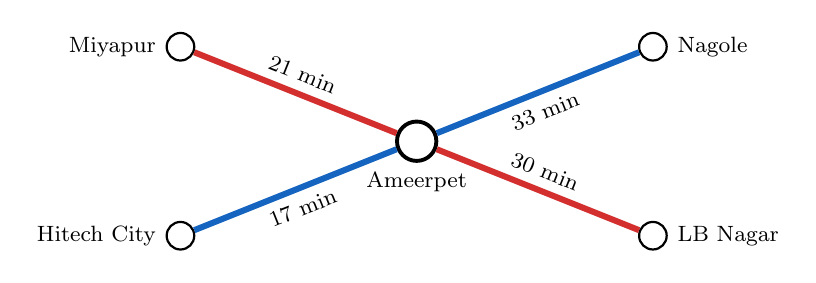
\begin{tikzpicture}[
  st/.style={circle,draw,thick,fill=white,minimum size=0.35cm,inner sep=0pt},
  lbl/.style={font=\footnotesize},
  every edge/.style={draw,line width=2.2pt}]
  \node[st,label={[lbl]left:Miyapur}] (m) at (0,1.2) {};
  \node[st,draw=black,line width=1.4pt,minimum size=0.5cm,label={[lbl]below=3pt:Ameerpet}] (a) at (3,0) {};
  \node[st,label={[lbl]right:LB Nagar}] (l) at (6,-1.2) {};
  \node[st,label={[lbl]left:Hitech City}] (h) at (0,-1.2) {};
  \node[st,label={[lbl]right:Nagole}] (n) at (6,1.2) {};
  \draw[metrored,line width=2.2pt] (m) -- node[lbl,above,sloped,text=black]{21 min} (a) -- node[lbl,above,sloped,text=black]{30 min} (l);
  \draw[metroblue,line width=2.2pt] (h) -- node[lbl,below,sloped,text=black]{17 min} (a) -- node[lbl,below,sloped,text=black]{33 min} (n);
\end{tikzpicture}\\[0.2em]
{\footnotesize A tiny piece of the network. Ameerpet is an \emph{interchange}: two lines meet there.\ (Times simplified.)}
\end{center}

``Find the fastest route'' now becomes a well-known computer science problem:
\emph{find the cheapest path between two nodes}. The classic answer is
\textbf{Dijkstra's algorithm}. Here is a complete, beginner-sized version you can run:

\begin{lstlisting}[language=Python]
import heapq

graph = {
    "Miyapur":     [("Ameerpet", 21)],
    "Hitech City": [("Ameerpet", 17)],
    "Ameerpet":    [("Miyapur", 21), ("Hitech City", 17), ("LB Nagar", 30)],
    "LB Nagar":    [("Ameerpet", 30)],
}

def dijkstra(graph, start, goal):
    queue = [(0, start, [start])]      # (minutes so far, station, path)
    visited = set()
    while queue:
        minutes, station, path = heapq.heappop(queue)   # always the closest one
        if station == goal:
            return minutes, path
        if station in visited:
            continue
        visited.add(station)
        for next_station, cost in graph[station]:
            heapq.heappush(queue, (minutes + cost, next_station, path + [next_station]))
    return None

print(dijkstra(graph, "Miyapur", "Hitech City"))
# (38, ['Miyapur', 'Ameerpet', 'Hitech City'])
\end{lstlisting}

The trick is the \textbf{priority queue} (\texttt{heapq}): it always hands back the
station we can reach soonest, so the first time we pop the goal, we know no faster way exists.
Our real version in \file{algorithms/shortest.py} is the same idea, with our own heap
(\file{ds/heap.py}) instead of \texttt{heapq}.

\subsection{Why one station becomes several nodes}

The toy graph above has a problem: it cannot tell \emph{staying on the train} at Ameerpet
from \emph{getting off and changing lines}, which takes about 3 minutes of walking. So in
the real graph (\file{network/transit\_graph.py}) each station is split into several nodes:

\begin{itemize}
  \item \textbf{waiting} on the platform of one line (e.g.\ ``Ameerpet, Blue platform''), and
  \item \textbf{riding} a train of one line in one direction (e.g.\ ``Ameerpet, on a Red train towards LB Nagar'').
\end{itemize}

Edges then have \emph{kinds}: \textbf{board} (platform $\rightarrow$ train),
\textbf{ride} (station $\rightarrow$ next station), \textbf{transfer} (walk to another
line's platform, counts as one change) and \textbf{alight} (get off). This is called a
\emph{line-expanded graph}, and it lets us count line changes exactly.

\subsection{Trains do not wait for you: the timetable}

Trains leave every 4 minutes at peak hours and every 6--8 minutes otherwise, from 06:00 to
23:00 (\file{planner/timetable.py}). So the cost of a \emph{board} edge depends on the
clock: arrive at 08:43 and the next train is at 08:44, so you wait 1 minute. Because the cost
of an edge depends on the time you reach it, this is called \textbf{time-dependent} Dijkstra.

For ``arrive by 10:00'' we use \textbf{binary search}: try a departure time halfway through
the range, see if it arrives in time, and halve the range again, until we find the
\emph{latest} time you can leave.

\needspace{14\baselineskip}
\subsection{All the algorithms, in plain words}

\begin{tabularx}{\linewidth}{@{}>{\bfseries}l X@{}}
\toprule
Algorithm & Question it answers \\
\midrule
Dijkstra & What is the fastest route? \\
A* (``A-star'') & The same answer, but faster to compute: it uses the straight-line distance to the destination as a hint, so it looks in the right direction first. \\
BFS & What is the route with the fewest stations? (Every edge counts as 1.) \\
0-1 BFS & What is the route with the fewest line changes? (Edges cost 0 or 1.) \\
Yen's algorithm & What are the 2nd and 3rd best routes, which are genuinely different? \\
Pareto search & Show every sensible trade-off, e.g.\ ``fastest with 2 changes'' vs ``5 minutes slower but no change''. \\
Binary search & What is the latest time I can leave and still arrive by a deadline? \\
\bottomrule
\end{tabularx}

The \textbf{Algorithms} tab of the website runs them side by side and shows how many
nodes each one looked at. A* usually looks at far fewer nodes than Dijkstra, for the same answer.

\subsection{Data structures we built}

\begin{itemize}
  \item \textbf{Heap} (\file{ds/heap.py}) --- the priority queue that Dijkstra and A* use.
  \item \textbf{Trie} (\file{ds/trie.py}) --- a tree of letters for \emph{autocomplete}.
        Type \texttt{ame} and it walks A$\rightarrow$M$\rightarrow$E to find ``Ameerpet'' instantly,
        without checking all 57 names.
  \item \textbf{Edit distance} (\file{ds/fuzzy.py}) --- counts how many letter changes turn
        one word into another. ``Ameerpeth'' is 1 change away from ``Ameerpet'', so typos still work.
  \item \textbf{Graph} (\file{ds/graph.py}) --- a dictionary mapping each node to its list of edges.
\end{itemize}

\subsection{The AI part}

\textbf{Understanding the question} (\file{nlp/llm\_parser.py}). We send Gemini the question
together with the list of real stations, and ask it to reply in strict JSON:
\begin{lstlisting}[language=Python]
{"origin": "Ameerpet", "destination": "Hitech City",
 "mode": "fewest_transfers", "arrive_by": "10:00", "avoid": [], "language": "en"}
\end{lstlisting}
Gemini is good at landmarks (``Inorbit Mall'' $\rightarrow$ Durgam Cheruvu station) and at
Telugu or Hindi. But we \textbf{never trust it blindly}: every station name it returns is
checked against our station list, and unknown ones are dropped.

\textbf{The offline rule parser} (\file{nlp/rules.py}) always runs too. It uses plain Python
and regular expressions: words like \emph{from} or \emph{at} mark the start, \emph{to} or
\emph{reach} mark the destination, and patterns like ``before 10'' or ``by 9:30 am'' become
times. If Gemini is missing or leaves a field empty, these rules fill the gap.

\textbf{Explaining the answer} (\file{nlp/explain.py}). After the planner finds the route, we
give Gemini only the verified facts (lines, stations, times, fare) and ask for a short,
friendly explanation, with the instruction not to invent anything. Without Gemini, a
fill-in-the-blanks template writes the explanation instead.

\textbf{Safety switch.} If the API key is wrong, or Gemini fails 3 times in a row, the app
stops calling it for a while (a \emph{circuit breaker}) instead of making you wait.

\textbf{Streaming.} Like ChatGPT, the answer appears word by word. The server sends small
pieces as soon as they are ready, using \emph{Server-Sent Events}, and the page types them out.

\section{Following one question through the code}

What happens when you type \emph{``cheapest way from LB Nagar to Miyapur''} and press Ask:

\begin{enumerate}
  \item The browser (\file{web/static/app.js}) sends the text to \texttt{POST /api/ask/stream}.
  \item Flask (\file{web/api.py}) receives it and calls \texttt{Assistant.ask\_stream} in \file{nlp/assistant.py}.
  \item The assistant \emph{understands} the text: Gemini and the rule parser each produce a
        \texttt{TripQuery} (from, to, mode, time), and the two are combined.
  \item Station names are matched to real stations by \file{nlp/stations.py} (trie + typo matching).
  \item \texttt{RoutePlanner.plan} (\file{planner/planner.py}) runs A* on the transit graph,
        using the timetable for waiting times.
  \item The result is turned into readable steps, and the fare is looked up
        (\file{planner/itinerary.py}).
  \item The explainer streams a friendly explanation back, piece by piece.
  \item The page shows the steps, types out the explanation and draws the route on the map.
  \item The search is saved in the SQLite \texttt{search\_log} table.
\end{enumerate}

\section{Python concepts you will meet in the code}

\begin{tabularx}{\linewidth}{@{}>{\bfseries}l X >{\ttfamily\small\color{accent}}l@{}}
\toprule
Concept & What it means & \normalfont\textbf{Example file} \\
\midrule
Packages and modules & A folder with \texttt{\_\_init\_\_.py} is a package; each \texttt{.py} file is a module. & src/routemate/ \\
Classes & Group data and the functions that use it. & planner/planner.py \\
\texttt{@dataclass} & A short way to write classes that mainly hold data. & ds/graph.py \\
Type hints & \texttt{def f(x: int) -> str} documents what goes in and out. & everywhere \\
Generators (\texttt{yield}) & A function that hands back results one at a time; used for streaming. & nlp/assistant.py \\
Decorators & \texttt{@api.get("/health")} tells Flask which URL a function answers. & web/api.py \\
\texttt{sqlite3} & Python's built-in database module. & db.py \\
\texttt{json} & Read and write JSON data. & db.py \\
Exceptions & \texttt{raise PlanningError(...)} reports problems like ``no train at this hour''. & planner/planner.py \\
pytest & Functions named \texttt{test\_...} with \texttt{assert} lines. & tests/ \\
\bottomrule
\end{tabularx}

\section{How we know it works: the tests}

The \file{tests/} folder has 117 tests that run in about 3 seconds. The most interesting ones
check our algorithms against \textbf{brute force}: on random graphs, a slow but obviously
correct method (like trying every possible path) must give exactly the same answer as our
fast algorithm. Other tests check the planner (``step times add up to the total''), the AI
layer (using a \emph{fake} Gemini so no internet is needed) and the website (through
Flask's test client).

\section{Glossary}

\begin{description}[itemsep=0.1em]
  \item[Node / edge] A dot and a connecting line in a graph.
  \item[Interchange] A station where lines meet: Ameerpet, MG Bus Station, Parade Ground.
  \item[Headway] Minutes between two trains on the same line.
  \item[Heuristic] A smart guess that guides a search (A* uses straight-line distance).
  \item[API] A web address that returns data (JSON) instead of a web page, e.g.\ \texttt{/api/route}.
  \item[API key] A secret password that lets our app use Gemini.
  \item[JSON] A text format for data that looks like Python dictionaries and lists.
  \item[LLM] Large Language Model, the kind of AI that Gemini is.
  \item[Fallback] What we do when the preferred option fails (rules instead of Gemini).
\end{description}

\section{Get familiar: things to try}

\begin{enumerate}
  \item Ask: \emph{Uppal to Jubilee Hills Check Post at 6pm, avoid Ameerpet}. Then ask the follow-up \emph{what if I want the fastest?}
  \item In the Plan tab, pick ``Arrive by'' 10:00 and see the latest time you can leave.
  \item Open the Algorithms tab and compare how many nodes Dijkstra and A* settle.
  \item Visit \url{http://127.0.0.1:5050/api/route?from=Ameerpet&to=Uppal} to see the raw JSON.
  \item Misspell a station (``dilsuknagar'') and watch it still work.
  \item Change a headway in \file{data/hyderabad\_metro.json}, restart the server and see the waiting times change.
  \item Break something on purpose, run \texttt{uv run pytest}, and see which test catches it.
\end{enumerate}

\end{document}
